%Innholdet til selveste presentasjon
%Titel page
\begin{frame}[t,plain]
    \titlepage
\end{frame}

% her kan du plassere en QR kode som lar folk laste ned filen (filene er i images folder)
\subsection*{Download the PDF}
\begin{frame}{Script and Presentation}
    \begin{figure}
        \centering
        
\includegraphics[height = 4.9cm]{qrcode.png}
        \caption{https://github.com/Swi005/Book-of-Magne/tree/v2023}
        \label{fig:qrcode}
    \end{figure}
\end{frame}

%===============================================
%Innholdet til selveste presentasjonen
\section{Programming Languages}
\subsection{What is a Programming Language?}
\begin{frame}{\textbf{What is a Programming Language?}}
    A Programming language is ...
    \begin{itemize}[<+->]
        \item used to tell a computer what to do
        \item usually artificial
    \end{itemize}
\end{frame}

\subsection{Grouping Languages by Domain}
\begin{frame}{\textbf{Grouping Languages by domain}}
    Languages are usually grouped into two categories when based on their specificity
    \begin{itemize}[<+->]
        \item DSLs, small,  targeted at specific problems. Internal/embedded vs external 
        \item GPLs, large, many uses.
    \end{itemize}
\end{frame}
\subsection*{Grouping Languages by Domain}
\begin{frame}{\textbf{Grouping Languages by domain}}
    \begin{figure}[!h]
        \centering
        \begin{tabular}{|c|c|c|c|}
            \hline
            \textbf{Characteristic} &\textbf{DSL } &\textbf{GPL}\\
            \hline
            \textbf{Domain} & Small and well-defined domain & Generality, many use cases\\
            \hline
            \textbf{Size} &Small ASTs & Large ASTs, often user extensible\\
            \hline
            \textbf{Lifespan} &As long as their domain &years to decades\\
            \hline
            \textbf{Extensibility} &Usually not extendible & Extendable\\
            \hline
        \end{tabular}%
        \caption{Comparison between GPLs and DSLs}
    \end{figure}%
\end{frame}


\subsection{Syntax and Semantics}
\begin{frame}{\textbf{Syntax and Semantics}}
    \begin{block}{Definition}
        All languages consist of two parts
        \begin{itemize}[<+->]
            \item \textbf{Syntax} - Defines shape
            \item \textbf{Semantics} - Defines meaning
        \end{itemize}
    \end{block}
    \Large
    Syntax is defined by a grammar.\\
    Grammar is not covered in this course :)
\end{frame}


\subsection{Meta Programming}
\begin{frame}{\textbf{Meta Programming}}
    A metaprogram is a program that works on \textit{other} programs.\\
    Compilers and Interpreters are examples of metaprograms
    \begin{block}{Definition}
        \begin{itemize}
            \item \textbf{Object Language} - Langage that gets compiled/interpreter
            \item \textbf{Meta Language} - Language used to implement the compiler/interpreter
        \end{itemize}
    \end{block}
\end{frame}

\subsection{Sum of Products}
\begin{frame}[fragile]{\textbf{Sum of Products}}
    \begin{figure}
        \centering
        \begin{minipage}{.5\textwidth}
            \begin{lstlisting}[language=Haskell]
    data SomeType = A Bool Bool Bool
                    | B Bool
                    | C
            \end{lstlisting}
        \end{minipage} 
    \end{figure}
    
    \begin{examples}
        \begin{equation*}
            \underbrace{(\text{Bool} \times \text{Bool} \times \text{Bool})}_{A} + \underbrace{\text{Bool}}_{B} + \underbrace{1}_{C}
        \end{equation*}
        \texttt{Bool} is either \texttt{True} or \texttt{False}.\\
        The total number of values of type SomeType is $8 + 2 + 1 = 11$.
    \end{examples}
\end{frame}

\subsection*{Sum of Products}
\begin{frame}[fragile]{\textbf{Sum of Products}}
    \begin{figure}
        \centering
        \begin{minipage}{\textwidth}
            \centering
            \begin{lstlisting}[language=Java]
    interface SomeType {}
    class A implements SomeType {
        boolean a;
        boolean b;
        boolean c ;
    }
    class B implements SomeType {
        boolean a;
    }
    class C implements SomeType {
    }
            \end{lstlisting}
        \end{minipage}
        \caption{Sum of Products in Java}
    \end{figure}
\end{frame}

\subsection*{Q\&A}
\begin{frame}{Questions?}
    \begin{figure}
        \centering
        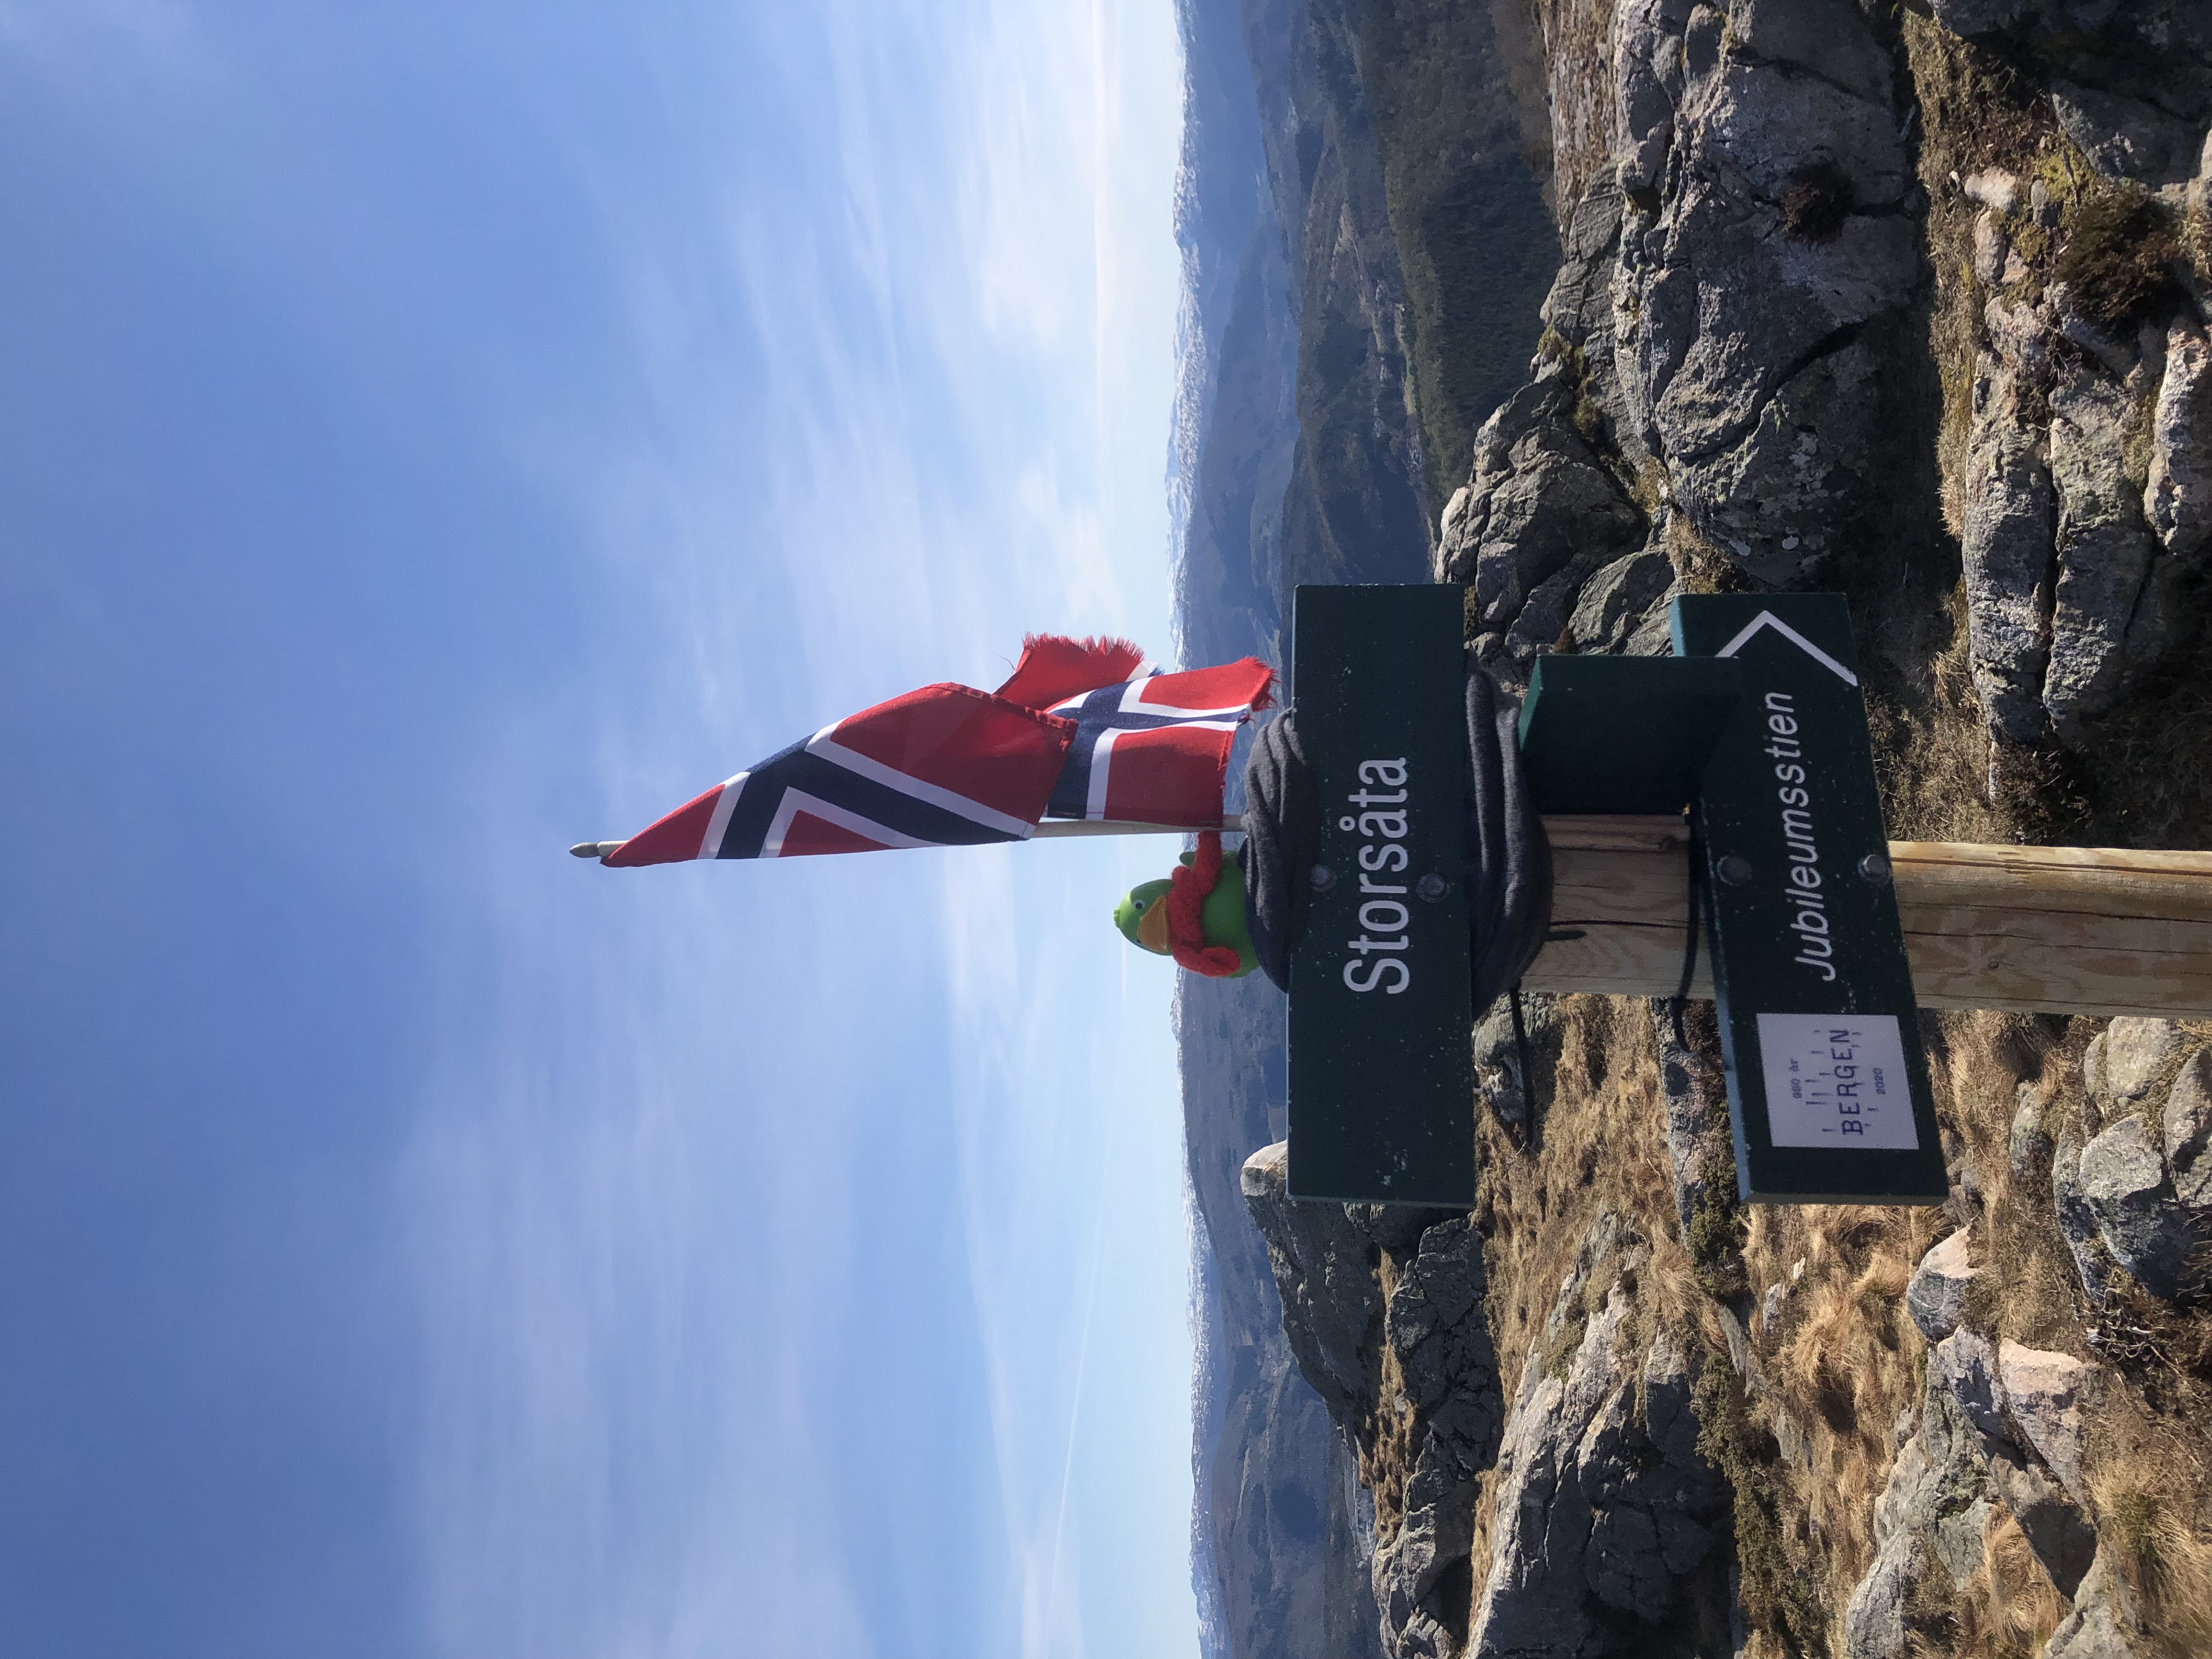
\includegraphics[height = 4.9cm]{guillaume2.jpg}
    \end{figure}
\end{frame}



\section{Interpreters}
\subsection{Compiler vs. Interpreters}
\begin{frame}{\textbf{Compiler vs. Interpreters}}
    \begin{figure}
        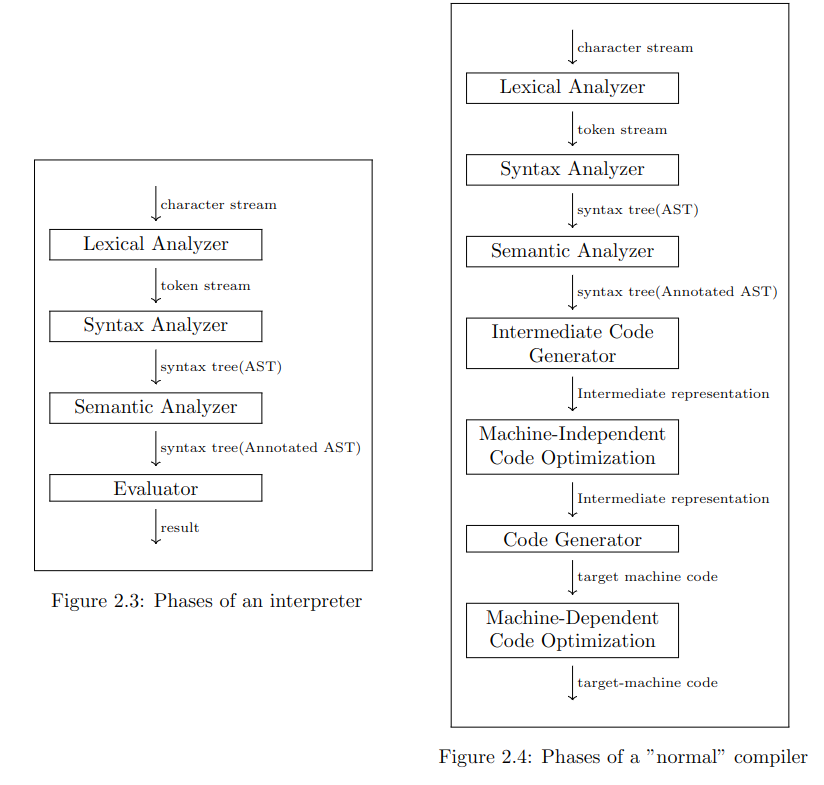
\includegraphics[scale=0.30]{Interpreter vs. Compiler.png}   
    \end{figure}
\end{frame}


\begin{frame}{\textbf{NB! IMPORTANT}}
    \begin{alertblock}{Compilers vs Interpreters!}
        We often end up using the term Compiler to talk about both Compilers and Interpreters, this is because they are very similar.\\
        This course deals exclusively with interpreters so unless stated otherwise assume that we are talking about interpreters.
    \end{alertblock}
    \begin{alertblock}{Expr vs AST}
        \begin{itemize}
            \item \textbf{Expr}: Expressions are terms that can be evaluated to a value, e.g. \texttt{1+2*3}
            \item \textbf{Stmt}: Statements are terms that are executed and result in a change of state. e.g. \texttt{var a = 1+2*3}
        \end{itemize}
    \end{alertblock}
\end{frame}

\subsection{Phases of an Interepreter}
\begin{frame}[fragile]{\textbf{Lexical Analysis}}
    \begin{block}{}
        \textbf{Lexical Analysis} breaks up strings into tokens. Also called a tokenizer.
    \end{block}
    \begin{example}
        \begin{figure}
            \centering
            \Large
            \begin{align*}
                (1+2)*13
            \end{align*}
        \end{figure}
        This gets tokenized into 
        \begin{lstlisting}[language=Haskell]
    ["(","1","+",2",")","*","13"]
        \end{lstlisting}
    \end{example}
\end{frame}
\subsection*{Phases of an Interepreter}
\begin{frame}{\textbf{Syntax Analyser}}
    \begin{example}
        \begin{figure}
            \centering
            \adjustbox{scale=0.7,center}{%
            \begin{tikzcd}
                \node[] (e0) {expr};
                \node[below left = of e0] (e1) {expr};
                \node[below left = of e1] (e11) {"("};
                \node[below = of e1] (e12) {expr};
                \node[below right = of e1] (e13) {")"};
                \node[below left = of e12] (e121) {number};
                \node[below = of e121] (e1211) {"1"};
                \node[below = of e12] (e122) {"+"};
                \node[below right = of e12] (e123) {number};
                \node[below = of e123] (e1231) {"2"};
                \node[below = of e0] (e2) {"*"};
                \node[below right = of e0] (e3) {number};
                \node[below = of e3] (e31) {"13"};
        
                \draw (e0) edge (e1)
                    (e0) edge (e2)
                    (e0) edge (e3)
                    (e1) edge (e11)
                    (e1) edge (e12)
                    (e1) edge (e13)
                    (e12) edge (e121)
                    (e12) edge (e122)
                    (e12) edge (e123)
                    (e121) edge (e1211)
                    (e123) edge (e1231);
        
            \end{tikzcd}
            }
        \end{figure}
    \end{example}
\end{frame}

\begin{frame}{\textbf{AST}}
    \begin{example}
        \begin{figure}[!h]
            \centering
            \adjustbox{scale=1,center}{%
            \begin{tikzcd}
                \node[] (e0) {\texttt{Mult}};
                \node[below left = of e0] (e1) {\texttt{Add}};
                \node[below left = of e1] (e11) {\texttt{1}};
                \node[below right = of e1] (e12) {\texttt{2}};
                \node[below right = of e0] (e2) {\texttt{13}};
        
                \draw (e0) edge (e1)
                    (e0) edge (e2)
                    (e1) edge (e11)
                    (e1) edge (e12);
            \end{tikzcd}
            }
        \end{figure}
    \end{example}
\end{frame}

\subsection{Semantic Analysis}
\begin{frame}{\textbf{Semantic Analyisis}}
    Semantic analysis lets us find out if the program is wellformed at find bugs at compile time, instead of at runtime.
    It also annotates the AST with certain information that's necessary for execution.

    \begin{block}{Wellformedness}
        For a program to be wellformed, we need to check for the following:
        \begin{itemize}
            \item \textbf{Type correctness}: The types of expressions in the program are correct.
            \item \textbf{Scope correctness}: The variables used in the program are declared.
            \item \textbf{Flow correctness}: The program is not stuck in an infinite loop.
            \item and more\dots
        \end{itemize}
        The first point is checked by a \textbf{type checker}.
    \end{block}
\end{frame}

\subsection{Type Checking}
\begin{frame}[fragile]{\textbf{Type Checking}}
    
    \begin{example}
        AST
        \lstinputlisting[language=Haskell, firstline=2, lastline=11]{examples/typecheck/typecheck.hs}
    \end{example}
\end{frame}
\subsection*{Type Checking}
\begin{frame}[fragile]{\textbf{Type Checking}}
    \begin{example}
        Types
        \lstinputlisting[language=Haskell, firstline=12, lastline=12]{examples/typecheck/typecheck.hs}
    \end{example}
\end{frame}

\begin{frame}[fragile]{\textbf{Type Checking}}
    \begin{example}
        \lstinputlisting[language=Haskell, firstline=14, lastline=21]{examples/typecheck/typecheck.hs}
    \end{example}
\end{frame}

\begin{frame}[fragile]{\textbf{Type Checking}}
    \begin{example}
        \lstinputlisting[language=Haskell, firstline=23, lastline=26]{examples/typecheck/typecheck.hs}
    \end{example}
\end{frame}

\begin{frame}[fragile]{\textbf{Type Checking}}
    \begin{example}
        \lstinputlisting[language=Haskell, firstline=28, lastline=31]{examples/typecheck/typecheck.hs}
    \end{example}
\end{frame}

\begin{frame}[fragile]{\textbf{Type Checking}}
    \begin{example}
        \lstinputlisting[language=Haskell, firstline=33, lastline=36]{examples/typecheck/typecheck.hs}
    \end{example}
\end{frame}

\begin{frame}[fragile]{\textbf{Type Checking}}
    \begin{example}
        \lstinputlisting[language=Haskell, firstline=38, lastline=41]{examples/typecheck/typecheck.hs}
    \end{example}
\end{frame}

\begin{frame}[fragile]{\textbf{Type Checking}}
    \begin{example}
        \lstinputlisting[language=Haskell, firstline=43, lastline=46]{examples/typecheck/typecheck.hs}
    \end{example}
\end{frame}

\begin{frame}[fragile]{\textbf{Type Checking}}
    \begin{example}
        \lstinputlisting[language=Haskell, firstline=48, lastline=48]{examples/typecheck/typecheck.hs}
    \end{example}
\end{frame}

\begin{frame}[fragile]{\textbf{Type Checking}}|
    \begin{example}
        \lstinputlisting[language=Haskell, firstline=50]{examples/typecheck/typecheck.hs}
    \end{example}
\end{frame}
\subsection*{Q\&A}
\begin{frame}{Questions?}
    \begin{figure}
        \centering
        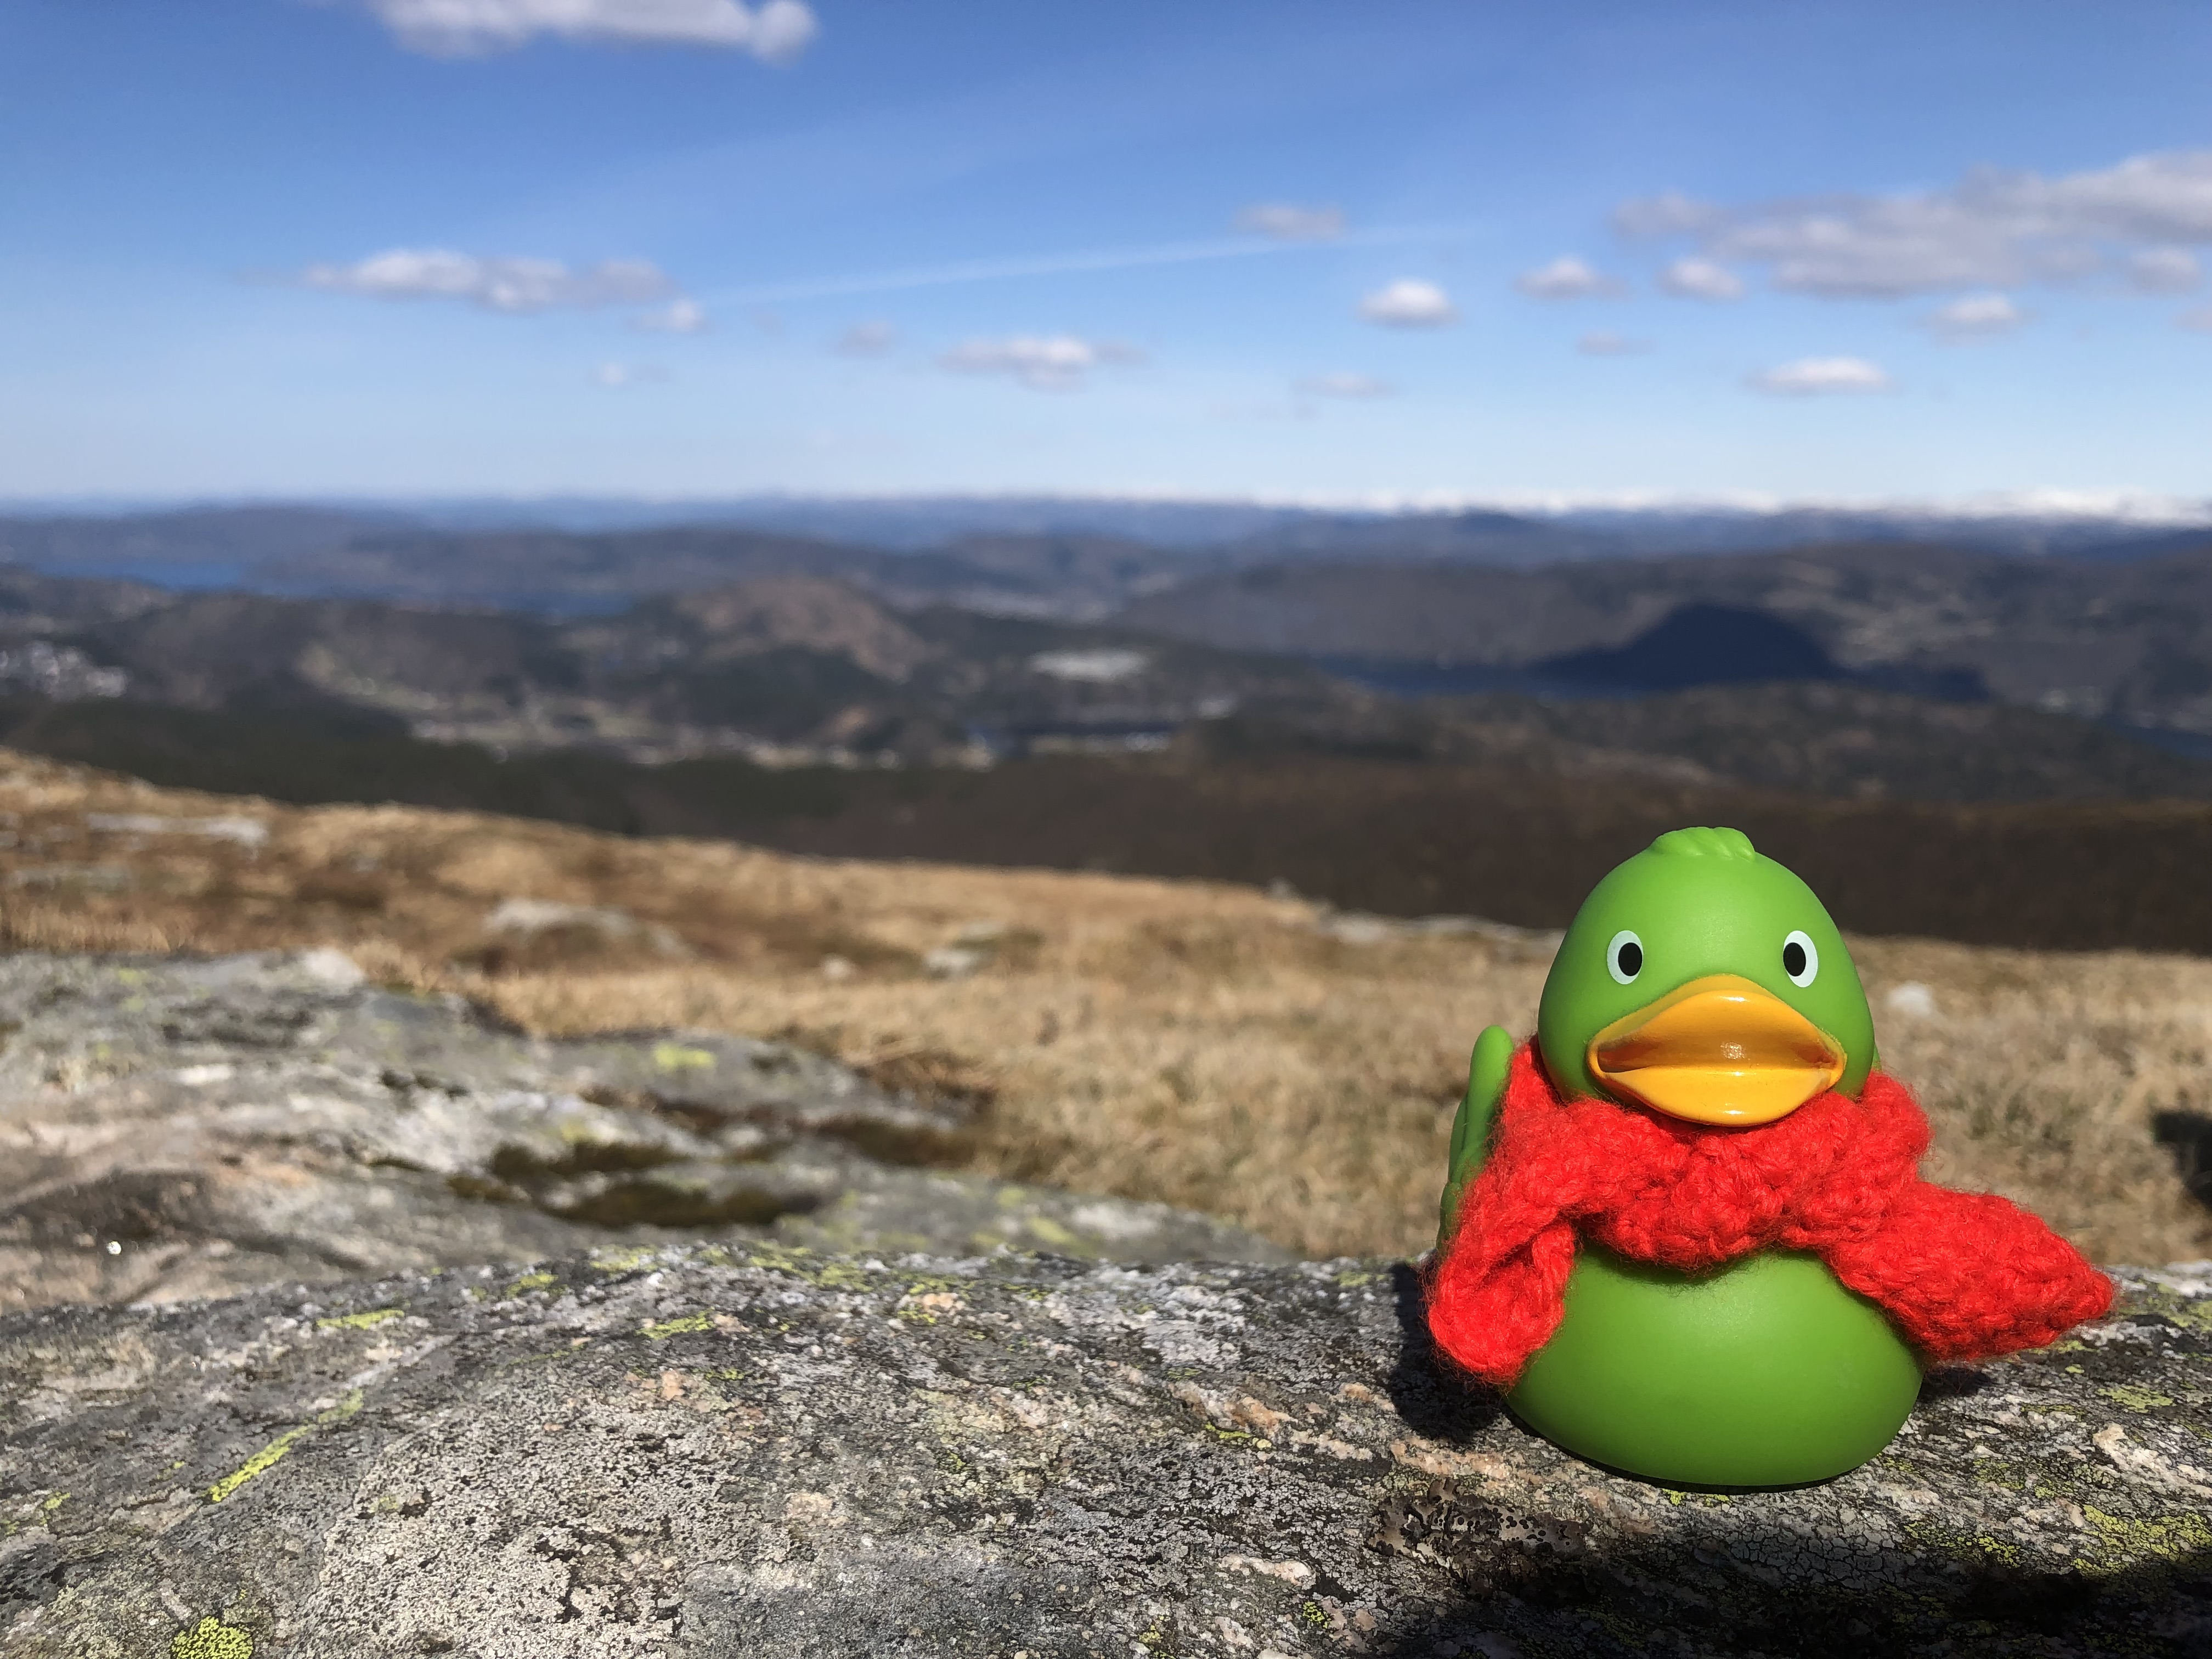
\includegraphics[height = 4.9cm]{guillaume3.jpg}
    \end{figure}
\end{frame}

\subsection*{Compiler vs. Interpreters}
\subsection{Phases of an Interepreter}
\subsubsection{Lexical Analyzer}
\subsubsection*{Static analyzer}
\subsubsection*{Semantic Analyzer}
\subsubsection*{Evaluator}
\subsection*{ASTs}
\subsection*{Type Checking}
\subsection*{Wellformedness}

\section{State}

\subsection{State}
\begin{frame}{\textbf{State}}
    The state is the place where the program stores its variables and data.
    \begin{block}{State}
        The state is divided up into two parts:
        \begin{itemize}
            \item \textbf{Enviroment}: The place where the program stores its variables.
                                        dictionary, where keys are variable names and values, are pointers to locations in the store. 
                                        The environment also contains the Free Pointer, which points to the next free location in memory.
            \item \textbf{Store}: The place where the program stores its data, aka Memory.
                                    The store is usually an array of values. Most often the values are bytes and types often take up multiple slots.
                                    Semantic analysis is used to determine the size of the types and to figure out addresses.
        \end{itemize}
    \end{block}
\end{frame}

\subsection{Scoping}
\begin{frame}{\textbf{Scoping}}
    Scoping is the process of determining where a variable is visible to the program.\\
    Scoping is usually divided into three different classes:
    \begin{itemize}
        \item \textbf{Runtime Scoping}
        \item \textbf{Static Scoping}
        \item \textbf{Dynamic Scoping}
    \end{itemize}
\end{frame}

\subsection*{Scoping}
\begin{frame}[fragile]{\textbf{Scoping}}
    \begin{example}
        \lstinputlisting[language=c,basicstyle=\ttfamily\tiny]{examples/scoping/scoping.c}
    \end{example}
\end{frame}



\subsection{Arrays}
\begin{frame}{\textbf{Arrays}}
    \begin{block}{Arrays}
        Arrays are a collection of elements of the same type.
        They're most often stored as a contiguous block of memory.\\
        Formula for accessing an element in an array:
        \begin{equation*}
            \texttt{foo[n]} = \texttt{\&foo} + n * \texttt{sizeof(T)}
        \end{equation*}
        \begin{itemize}
            \item \texttt{\&foo} is the pointer to the array
            \item \texttt{n} is the index of the element we want to access
            \item \texttt{sizeof(T)} is the size of type T in bytes
        \end{itemize}
    \end{block}    
\end{frame}

\subsection*{Arrays}
\begin{frame}[fragile]{\textbf{Arrays}}
    \begin{example}
        \begin{lstlisting}[language=c]
    int foo[5] = {1,2,3,4,5};
        \end{lstlisting}
    \end{example}
\end{frame}

%\begin{frame}{Arrays}
%    \begin{example}
%        \begin{figure}
%            \centering
%            \adjustbox{scale=0.4}{
%                \begin{bytefield}{8}
%                    \begin{rightwordgroup}{\texttt{foo} is a pointer to the array at \texttt{0x00}}
%                        \memsection{0xff}{}{1}{\texttt{foo}}
%                    \end{rightwordgroup}\\
%                    \memsection{0xfe}{}{4}{...}\\
%                    \begin{rightwordgroup}{The actual array}
%                        \memsection{0x13}{}{4}{5}\\
%                        \memsection{0x0f}{}{4}{4}\\
%                        \memsection{0xb}{}{4}{3}\\
%                        \memsection{0x08}{}{4}{2}\\
%                        \memsection{0x04}{0x00}{4}{1}
%                    \end{rightwordgroup}
%                \end{bytefield}
%            }
%        \end{figure}
%    \end{example}
%\end{frame}

\begin{frame}{\textbf{Multidimensional Arrays}}
    Multidimensional arrays are arrays of arrays.
    \begin{block}{Multidimensional Arrays}
        There are two main ways of storing multidimensional arrays:
        \begin{itemize}
            \item \textbf{Array of Pointers}: Each element in the array is a pointer to another array somewhere else in memory.
            \item \textbf{Contiguous Block}: The entire multidimensional array is stored as a contiguous block of memory. Where each row is stored sequentially.
        \end{itemize}
    \end{block}
\end{frame}

\begin{frame}{\textbf{Multidimensional Arrays}}
    \begin{block}{Forumla for Contiguous Block}
        \begin{equation*}
            \texttt{bar[i][j]} = \texttt{\&bar} + i * \texttt{length(row)} + j * \texttt{sizeof(T)}
        \end{equation*}
        where 
        \begin{itemize}
            \item \texttt{\&bar} is the pointer to the array
            \item \texttt{i} is the row index
            \item \texttt{j} is the column index
            \item \texttt{sizeof(T)} is the size of type T in bytes
            \item \texttt{length(row)} is the length of the row
        \end{itemize}
    \end{block}
\end{frame}

\begin{frame}[fragile]{\textbf{Multidimensional Arrays}}
    \begin{example}
        \begin{lstlisting}[language=c]
    int bar[][] = {
            {1,2},
            {3,4}
        };
        \end{lstlisting}
    \end{example}
\end{frame}

\subsection{Records}
\begin{frame}{\textbf{Records}}
    Records are a collection of elements of different types.
    Each element is called a field.\\
    \begin{block}{Records}
        Records are stored as a contiguous block of memory. With each field stored consecutively.\\
        To access a field in a record we need to know the offset of the field in the record.
    \end{block}
\end{frame}

\subsection*{Records}
\begin{frame}{\textbf{Records}}
    \begin{block}{Records}
        Formula for accessing a field in a record:
        \begin{equation*}
            \texttt{foo.bar} = \texttt{\&foo} + \texttt{offset(bar)}
        \end{equation*}
        where 
        \begin{itemize}
            \item \texttt{\&foo} is the pointer to the record
            \item \texttt{bar} is the field that we want to access
            \item \texttt{offset(bar)} is the offset of the field \texttt{bar} in the record
        \end{itemize}
    \end{block}
\end{frame}

\begin{frame}[fragile]{\textbf{Records}}
    \begin{example}
        \begin{lstlisting}[language=c]
    struct foo {
        int x; //Offset 0
        bool y; //Offset 4
        double z; //Offset 5
    };
        \end{lstlisting}
    \end{example}
\end{frame}

\begin{frame}{\textbf{Arrays of Records}}
    \begin{block}{Records}
        Formula for accessing a field of the nth element in an array of records:
        \begin{equation}
            \texttt{foo[n].bar} = \texttt{\&foo} + n * \texttt{sizeof(T)} + \texttt{offset(bar)}
        \end{equation}
        where 
        \begin{itemize}
            \item \texttt{\&foo} is the pointer to the array
            \item \texttt{n} is the index of the element we want to access
            \item \texttt{sizeof(T)} is the size of type T in bytes
            \item \texttt{bar} is the field that we want to access
            \item \texttt{offset(bar)} is the offset of the field \texttt{bar} in the record
        \end{itemize}
    \end{block}
\end{frame}

\subsection*{Q\&A}
\begin{frame}{Questions?}
    \begin{figure}
        \centering
        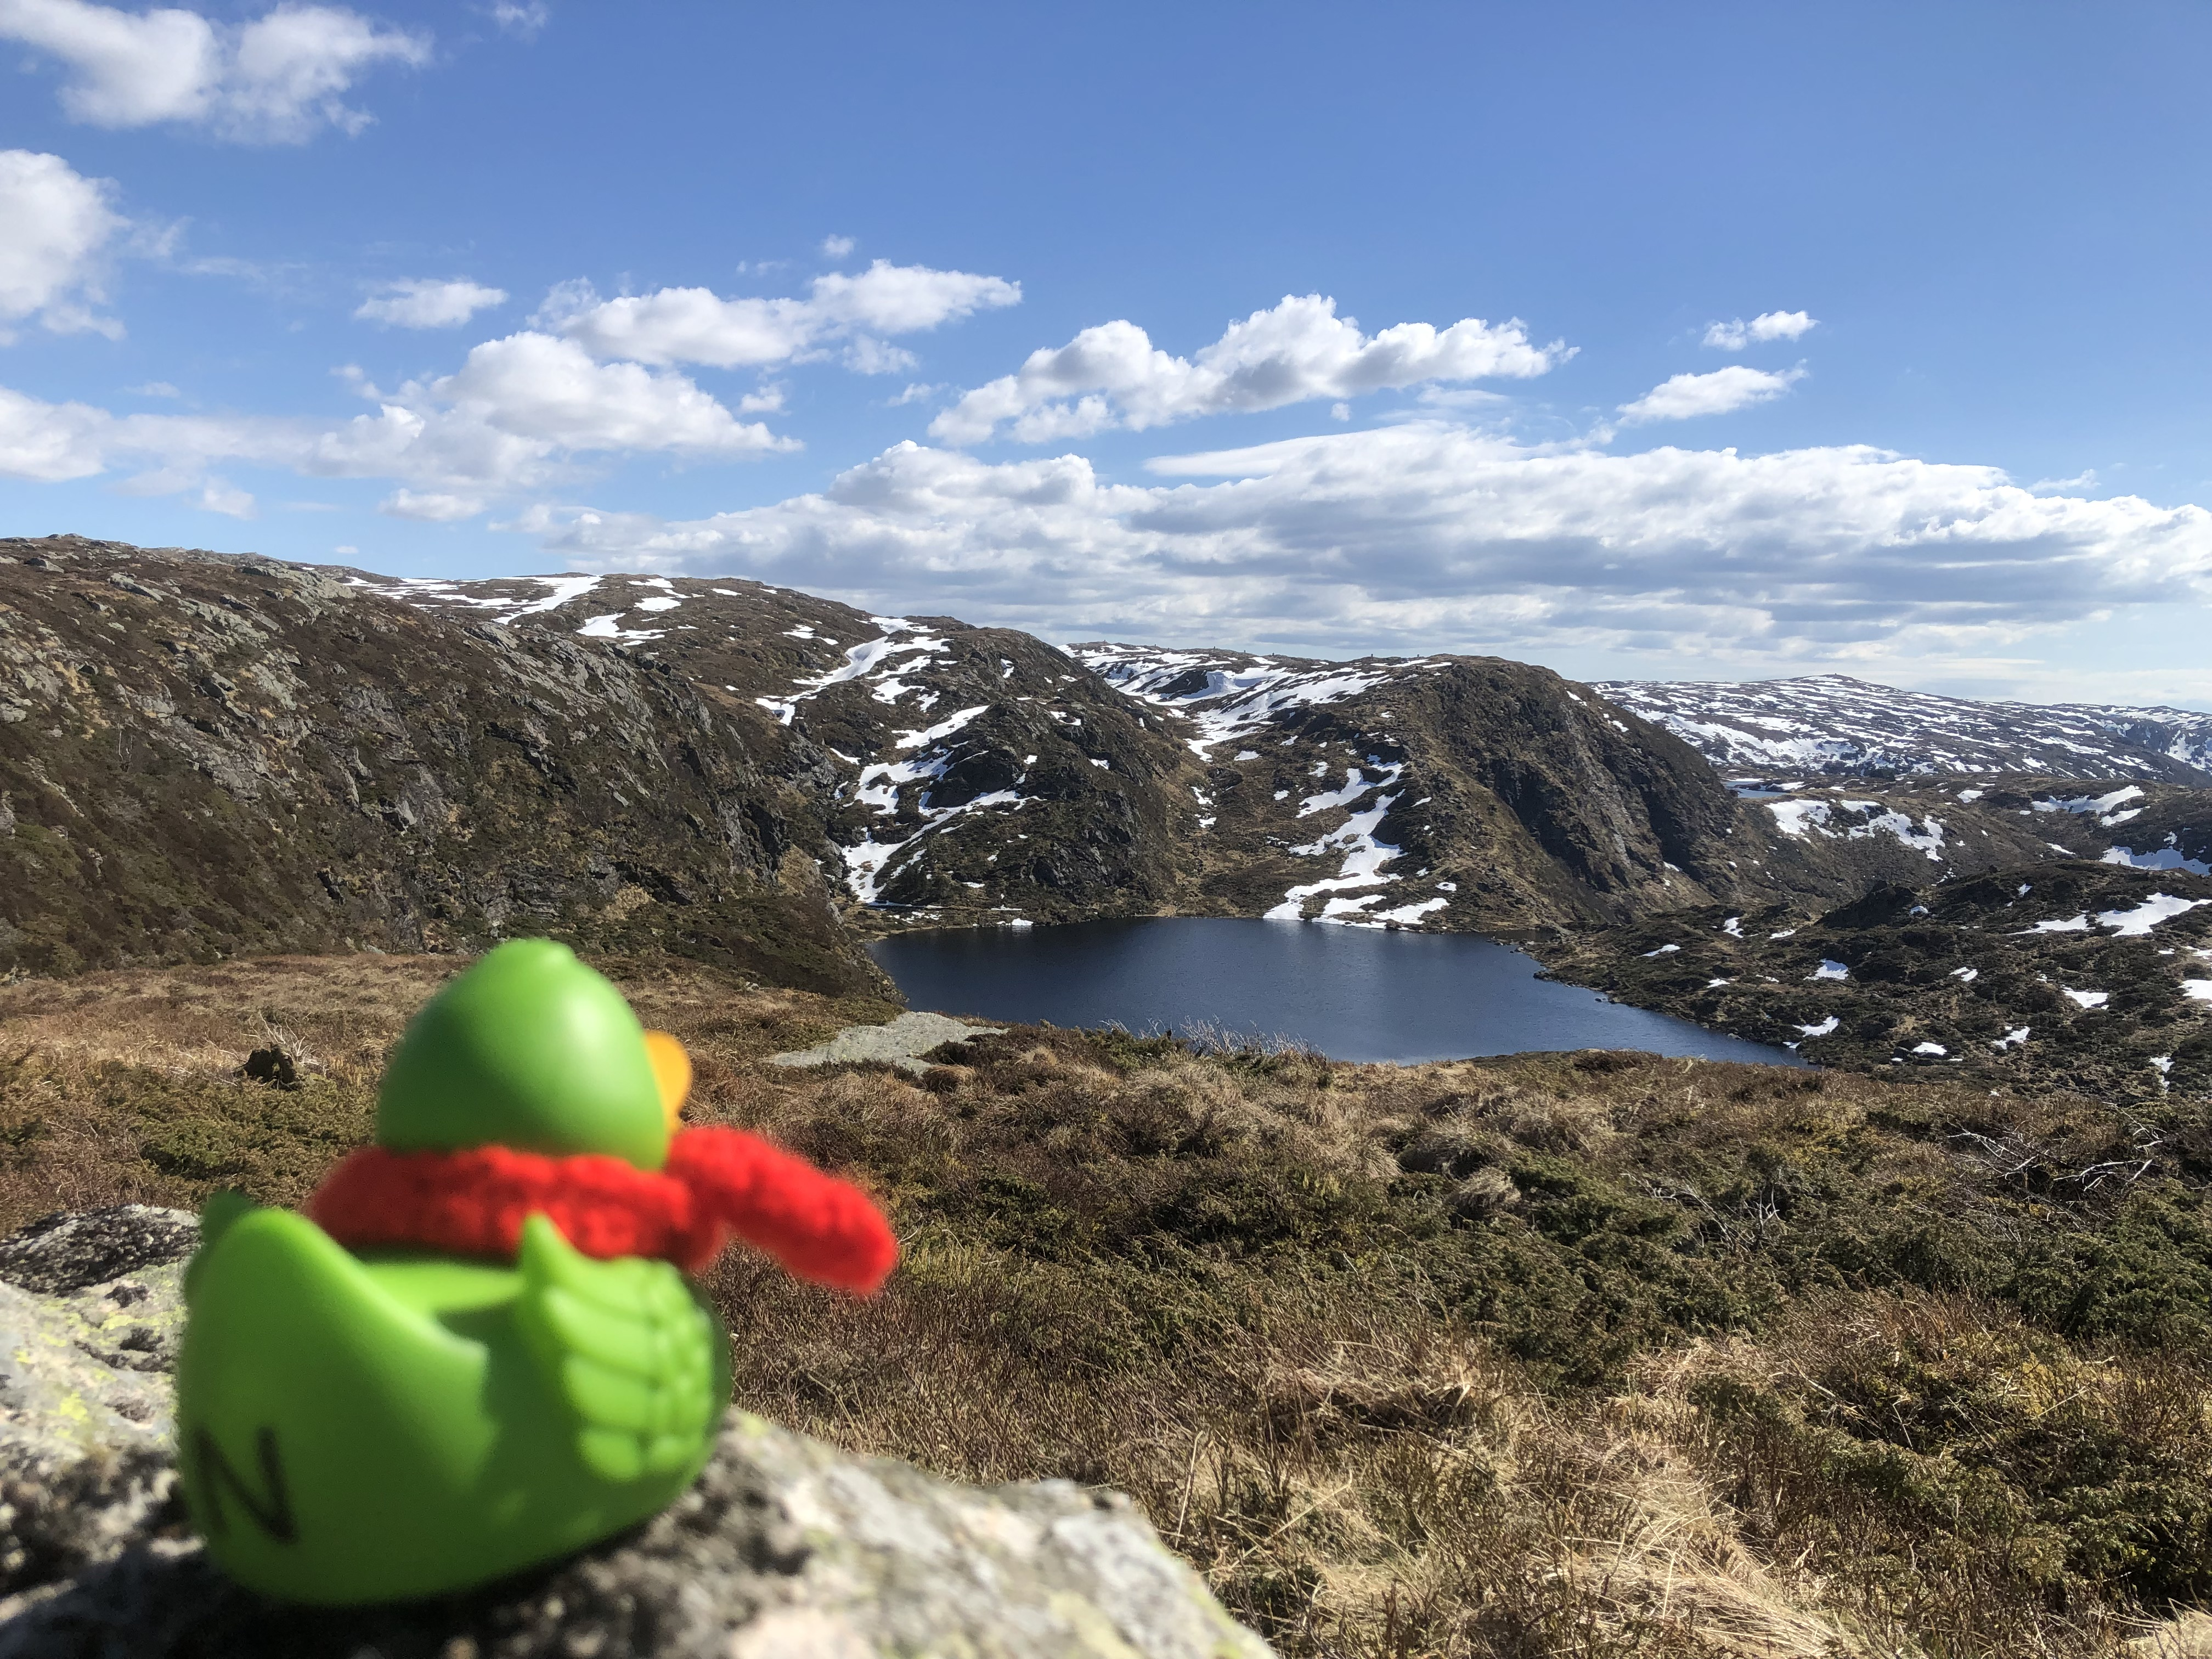
\includegraphics[height = 4.9cm]{guillaume4.jpg}
    \end{figure}
\end{frame}


\section{Procedures}

\subsection*{What is a Procedure}
\begin{frame}{\textbf{What is a Procedure}}
    \begin{itemize}
        \item Procedures are "programs within programs"
        \item Procedures have their own environment
    \end{itemize}
    \begin{alertblock}{Functions vs. Procedures}
        \begin{equation}
            \text{Functions} \neq \text{Procedures}
        \end{equation}
        Functions are expressions, procedures are statements.\\
        Very often same implementation.
    \end{alertblock}
\end{frame}

\subsection*{Anatomy of a procedure}
\begin{frame}{\textbf{Anatomy of a Procedure}}
    \begin{figure}
        \lstinputlisting[language=Pascal]{examples/anatomy.pipl}
    \end{figure}
    \begin{block}{Params}
        \begin{itemize}
            \item \textbf{OBS} - "read only"
            \item \textbf{UPD} - "read/write"
            \item \textbf{OUT} - "write only"
        \end{itemize}
    \end{block}
\end{frame}

\begin{frame}{\textbf{Declaration vs. Calling}}
    \begin{figure}
        \lstinputlisting[language=pascal, basicstyle=\ttfamily\tiny]{examples/ex1.pipl}
        \label{fig:ex1}
        \caption{Swap Procedure}
    \end{figure}
\end{frame}

\subsection*{Paramter Semantics}
\begin{frame}{\textbf{Parameter Semantics}}
    \Large
    Two types of parameter semantics:
    \begin{itemize}
        \item Reference semantics
        \item Copy semantics
    \end{itemize}
\end{frame}

\begin{frame}{\textbf{Reference Semantics}}
    \Large
    \begin{itemize}
        \item Parameters become aliased to arguments 
        \item Points to same memory address
        \item Unsafe, but sometimes useful
    \end{itemize}
\end{frame}
\begin{frame}{\textbf{Running a procedure with reference semantics}}
    \Large
    \begin{enumerate}[<+->]
        \item Get stackframe
        \item Wipe environment
        \item Add parameters to the environment with same address as arg
        \item run the procedure code
        \item restore the environment
    \end{enumerate}
\end{frame}
\begin{frame}{\textbf{Copy Semantics}}
    \Large
    \begin{itemize}
        \item Parameters are declared as variables and initialized with args' value
        \item Safer
        \item More intuitive behavior
        \item More complicated to implement
    \end{itemize}
\end{frame}

\begin{frame}{\textbf{Running a procedure with copy semantics}}
    
    \begin{enumerate}[<+->]
        \item Get stackframe
        \item Get values of args
        \item Wipe environment
        \item Add parameters to environment
        \item init those parameters with the arg values
        \item run the procedure code
        \item get the values of the parameters
        \item restore the environment
        \item copy the parameter values back to the args
    \end{enumerate}
\end{frame}


\subsection*{Reference semantics!}
\begin{frame}\textbf{{Reference semantics}}
    \lstinputlisting[language=Pascal]{examples/paramater semantics/copy/paramsem.pipl}
\end{frame}
\begin{frame}\textbf{{Reference semantics}}
    \lstinputlisting[language=Pascal]{examples/paramater semantics/copy/paramsem1.pipl}
\end{frame}
\begin{frame}\textbf{{Reference semantics}}
    \lstinputlisting[language=Pascal]{examples/paramater semantics/copy/paramsem2.pipl}
\end{frame}
\begin{frame}\textbf{{Reference semantics}}
    \lstinputlisting[language=Pascal]{examples/paramater semantics/copy/paramsem3.pipl}
\end{frame}

\subsection*{Example!}
\begin{frame}{\textbf{Swap example v2}}
    \lstinputlisting[language=Pascal]{examples/paramater semantics/paramsem.pipl}
\end{frame}

\subsection*{Copy semantics!}
\begin{frame}\textbf{{Copy semantics}}
    \lstinputlisting[language=Pascal]{examples/paramater semantics/reference/paramsem.pipl}
\end{frame}

\begin{frame}\textbf{{Copy semantics}}
    \lstinputlisting[language=Pascal]{examples/paramater semantics/reference/paramsem1.pipl}
\end{frame}
\begin{frame}\textbf{{Copy semantics}}
    \lstinputlisting[language=Pascal]{examples/paramater semantics/reference/paramsem2.pipl}
\end{frame}
\begin{frame}\textbf{{Copy semantics}}
    \lstinputlisting[language=Pascal]{examples/paramater semantics/reference/paramsem3.pipl}
\end{frame}




%\section*{Slutt}
\subsection*{Q\&A}
\begin{frame}{Questions?}
    \begin{figure}
        \centering
        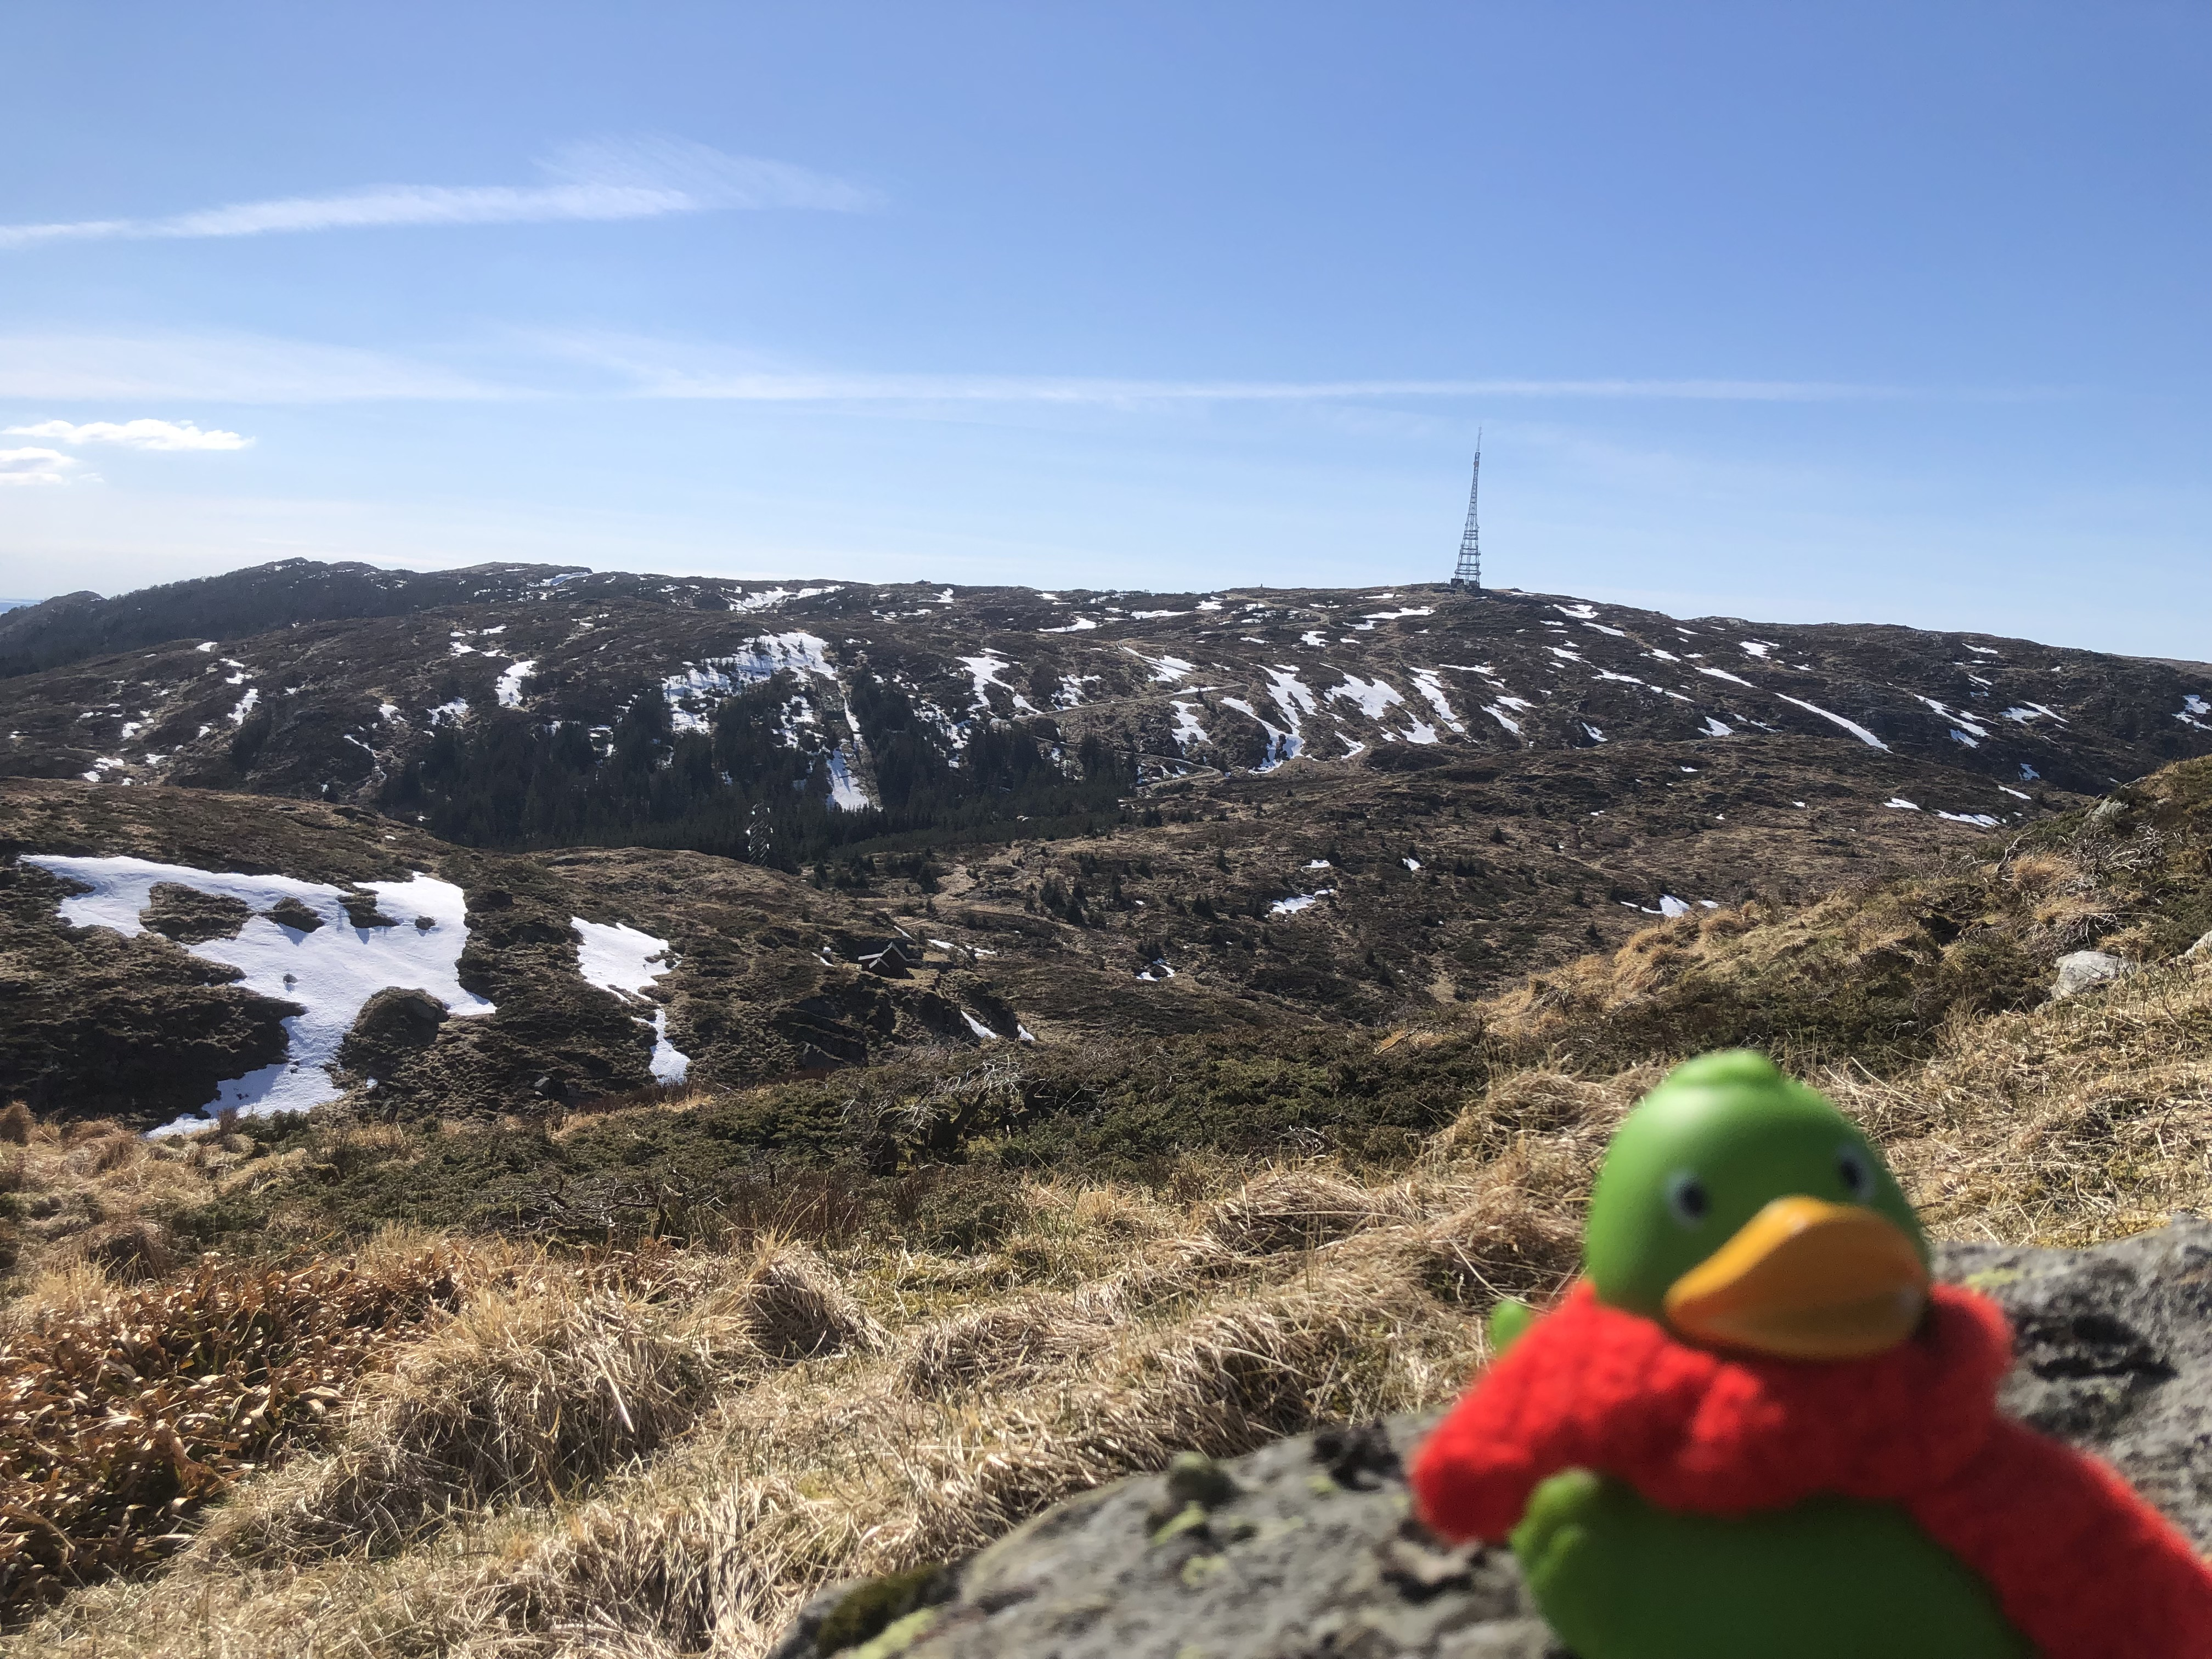
\includegraphics[height = 4.9cm]{guillaume5.jpg}
    \end{figure}
\end{frame}


\section{Signatures}
\chapter{Signatures}
So far we've defined all our operations as part of our AST. 
By introducing signatures into our compilers we can abstract away the implementation of our operations from the AST.
This allows us to change the implementation of our operations without changing the AST.
Before we can do this we need to talk a bit about the theory behind signatures and algebras

\section{A little bit of Theory}

\subsection{Signatures}
\gls{signature}s are a way to define a set of operations and their types.

Formaly a signature\footnote{also called an \textit{Interface}} is defined as $I = \langle S,F \rangle$ where
\begin{itemize}
    \item $S$ is a set of sorts(aka typenames), and
    \item $F$ is a set of function declarations $f: s_1, ..., s_n \rightarrow s$, for $s1, \dots, s_n, s \in S$
\end{itemize}
Signatures alone do not define any semantics, they are just a way to define which operations and types exist, but not what they do.
To define the semantics we need to define what we call an algebra.

Here's an example of a signature.
\begin{align*}
    Nat = \langle \{&N\},\\ 
                  \{&zero: N,\\
                    &succ: N \rightarrow N\} \rangle
\end{align*}

\subsection{Algebras}
An \gls{algebra} is a way to define the semantics of a signature.
An algebra assigns every sort to a domain and every function to a function on the domains.
An algebra $A$ for a signature $I = \rangle S,F \langle$ defines
\begin{itemize}
    \item a set $[\![s]\!]_A$ for every sort $s \in S$, and
    \item a total function $[\![f]\!]_A : [\![s_1]\!]_A \times ... \times [\![s_k]\!]_A \rightarrow [\![s]\!]_A$ for every  $(f: s_1, ... , s_k \rightarrow s) \in F$
\end{itemize}
It's possible to have multiple algebras for a signature.
Here are a couple of algebras for the $Nat$ signature.

\begin{align*}
    \alg{N}{A_1} &= \mathcal{N}\\
    \alg{zero}{A_1} &= 0\\
    \alg{succ}{A_1} &= \lambda n \mapsto n + 1\\
    &{}\\
    \alg{N}{A_2} &= \{1,2,7\}\\
    \alg{zero}{A_2} &= 2\\
    \alg{succ}{A_2} &= \lambda n \mapsto 7\\
\end{align*}



\section{Implementing Algebraic Specifications}
Integrating signatures and algebras into our interpreter means we can use Algebraic specification theory to formalize and reason about it.
It also lets us change the implementation of our operations without changing the AST and is one step towards user-defined types, and generic programming.

Lets take a look at how we can rewrite an interpreter to make use of signatures.

\begin{figure}[H]
    \lstinputlisting[language=Haskell, firstline=4]{figures/code/signatures/ex1/AST.hs}
    \label{fig:astx}
    \caption{Interpreter for a simple language}
\end{figure}

We do this by creating a new AST without any operations apart from Literals, Variables, and Function calls.
And instead of returning a \texttt{Int} we make it so that the AST can work for any \texttt{valuedomain}(FIgure \ref{fig:ast2}).

\begin{figure}[H]
    \lstinputlisting[language=Haskell, firstline=4, lastline=8]{figures/code/signatures/ex1/AST2.hs}
    \label{fig:ast2}
\end{figure}

We also change the evaluator to reflect this change. One major change(apart from the lack of operations) is that we now need to pass the algebra(\texttt{funmod}) to the evaluator.

\begin{figure}[H]
    \lstinputlisting[language=Haskell, firstline=11]{figures/code/signatures/ex1/AST2.hs}
    \label{fig:eval}
\end{figure}

Not that we've adapted the AST for signatures it's time to implement a signature for the operations we removed.

\begin{figure}[H]
    \lstinputlisting[language=Haskell, firstline=10, lastline=17]{figures/code/signatures/ex1/Intrinsics.hs}
    \label{fig:sig}
\end{figure}
You may have noticed one major change from the old AST. The old AST only worked on \texttt{Int}s, but we've added a second sort \texttt{Bool} to the signature.
Since Haskell only lets us use one type for the valuedomain we need to create a new type that can hold both \texttt{Int}s and \texttt{Bool}s.

\begin{figure}[H]
    \lstinputlisting[language=Haskell, firstline=20, lastline=20]{figures/code/signatures/ex1/Intrinsics.hs}
    \label{fig:valuedomain}
\end{figure}
\newpage

We then define our algebra for the functions in the signature.

\begin{figure}[H]
    \lstinputlisting[language=Haskell, firstline=22]{figures/code/signatures/ex1/Intrinsics.hs}
    \label{fig:alg}
\end{figure}

Now, there are some downsides to using signatures. For one we no longer get to use Haskell's built-in type system to check that we're using the right types.
That means that we need to implement and adapt our type checker to work with signatures.

\subsection{ADTs}
We've implemented Signatures in our interpreter, but we haven't given the user a way to define their own yet. 
We can do this by introducing \gls{adt} in our language.
Abstract Data Types are a way to define a type and its operations without exposing the implementation. \\
The best example of ADTs are probably Interfaces in Java.

Methods in Java Interfaces don't have any implementation\footnote{We'll conveniently ignore the existence of the \texttt{defaul} keyword.}, they just define the signature of the method.
This means that we can define a method in an interface and then implement it in multiple ways.
This is a very powerful tool for generic programming.

\begin{figure}[H]
    \lstinputlisting[language=Java, firstline=1]{figures/code/signatures/ADT/IStack.java}
    \label{fig:istack}
    \caption{ADT for a Stack}
\end{figure}

\newpage

Figure \ref{fig:stack} shows one implementation of \texttt{IStack}.

\begin{figure}[h]
    \lstinputlisting[language=Java, firstline=8, lastline=26]{figures/code/signatures/ADT/Stack.java}
    \label{fig:stack}
    \caption{Stack}
\end{figure}

Since ADTs don't specify an implementation it is perfectly valid for me to implement whatever I want as long as it has the same signature.
For example, I could implement \texttt{IStack} as a linked list instead of an array.
Or we could go a step further and observe that the only difference between stacks and queues is the behavior of \texttt{pop}.\\
So Figure \ref{fig:queue} is a totally valid implementation of the \texttt{Stack} ADT.

\begin{figure}[!h]
    \lstinputlisting[language=Java, firstline=7, lastline=26]{figures/code/signatures/ADT/Queue.java}
    \label{fig:queue}
    \caption{Queue}
\end{figure}
\section{Generic Programming}

\subsection{Concepts}


\section{Assertions}
\begin{frame}{\textbf{Assertions}}
    Assertions are statements that check if some predicate holds. 
    Assertions help make sure that a program is always in a valid state.
    If an assertion fails, a program crash is triggered.
    \begin{block}{Assertion Types}
        There is usually a couple of categories of assertions.
        \begin{itemize}
            \item \textbf{Pre-Condition}: assertions that must hold before a function or procedure is called. 
                                        Ensures that call is made with valid args.
            \item \textbf{Post Conditions}: assertions that must hold after a procedure/function.
                                           e.g. return type, valid result, etc.
            \item \textbf{Invariants}: assertions that must always hold, e.g some var is always above a certain value.
        \end{itemize}
    \end{block}
\end{frame}

%\section*{Slutt}
\begin{frame}
    \begin{center}
        \begin{Large}
        \textbf{Lykke til på eksamen!\\[5mm]
        Takk for meg :)}
        
        \end{Large}
        \begin{figure}
            \centering
            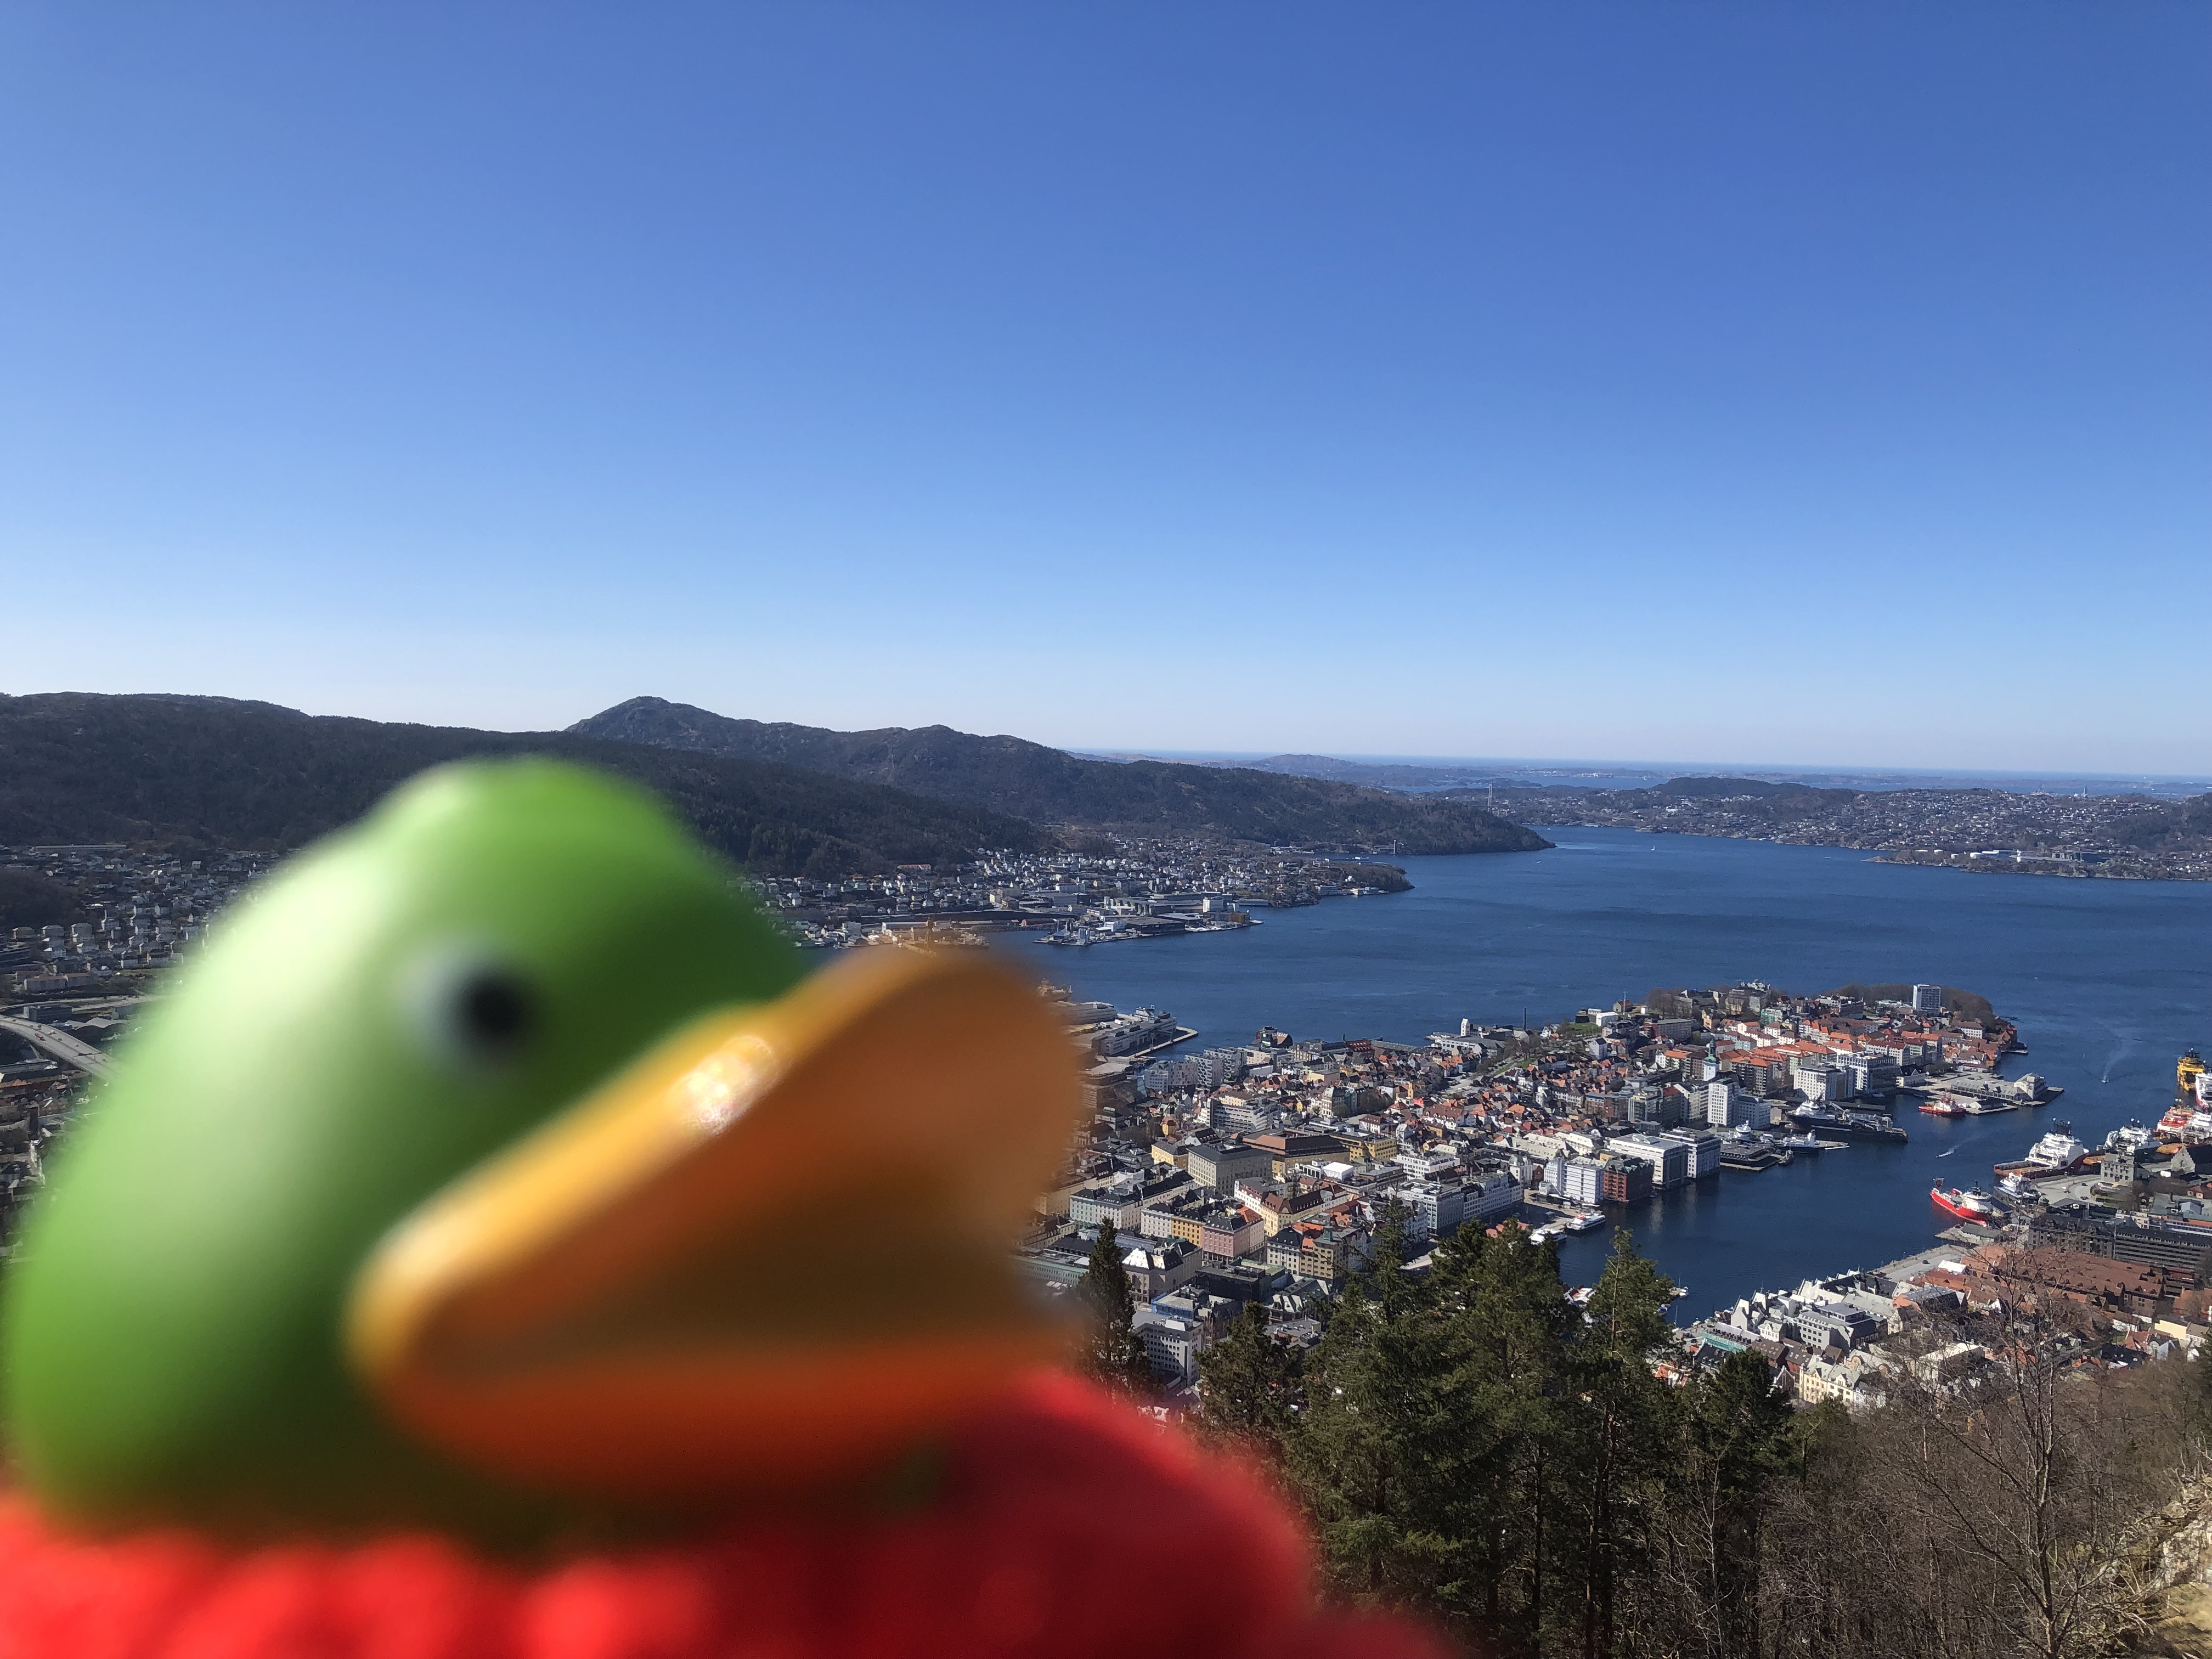
\includegraphics[height = 4.9cm]{guillaume10.jpg}
        \end{figure}
    \end{center}  
\end{frame}

